\chapter{Analysis}
\label{ch:analysis}

The acquisition of the data, as discussed in the previous chapter, was done using the NSCL DAQ \citep{nscl:_daq, prokop14:_nsclddas}. These files were converted into files compatible with ROOT \citep{brun97:_root}. In ROOT, calibrations, gates, and fitting were done. Fits of the peaks were also done in RADWARE \citep{radford00:_radware} and compared. RADWARE was used as the main fitting tool, as the built-in framework for the Fano factor \citep{fano47:_factor} created more consistent global fits, and a better estimate of the skew factors for the conversion electron spectra. Appendix \ref{chap:code} contains the analysis code used, and Appendix \ref{chap:macro} contains the ROOT macros discussed in the text.

\section{Fitting Spectra}
\label{sec:fitting}

Whenever possible, all data were fit using the same methodology. If another methodology needed to be used (as will be discussed in Section \ref{sec:upper_limit}) the methodology was tested. This was done by taking both fitting routines to the same peaks and comparing the results. If they were in agreement, the secondary method could be used where the primary method failed.

In a completely ideal scenario, the spectrum from an experiment should look like a series of delta functions. This is never the case in a real experiment, as detectors do not have infinite resolution, and do not cover an infinitesimal angle. Instead, an ideal experimental spectrum would have the peaks look like gaussian functions. The normal gaussian formula is 
\begin{equation}
    f(x) = he^{-\left(\frac{x-\mu}{\sqrt{2}\sigma}\right)^2}
    \label{eq:gaus}
\end{equation}
where $h$ is the height of the peak, $\mu$ is the centroid of the peak, and $\sigma^2$ is the variation of the peak. This function can be renormalized using the integral to give the area as a fitting parameter instead of the height as 

\begin{equation}
    A = h\sigma\sqrt{2\pi}
\end{equation}

The HPGe spectra were fitted using the gaussian formula. Fitting multiple peaks at once in a spectrum requires a secondary consideration: the Fano factor. The Fano factor is a measure of dispersion within a detector\citep{fano47:_factor}. It takes into account that the energy loss in the detector is not purely statistical, as the gaussian distribution would assume. This goes into the resolution of the detector, which is related to the energy of the particle being detected. As a result, the resolution changes with energy. This is reflected in the variation ($\sigma^2$) in the fit. To do this in ROOT, the fitting function must be written to reflect this information, tying the width of every peak together under certain assumptions. As there is not an iterative way to create such a function in ROOT for $x$ number of peaks, an individual fitting function must be written for each number $x$ of peaks to fit. This becomes exceedingly tedious. However, RADWARE has this energy adjustment built into the fitting code, allowing the correlation between peaks to be turned off if needed for up to 35 peaks. If there are background peaks that should not have a correlation, such as the case of a Compton peak, it can be turned off for individual peaks.

In the previous chapter, the results of the calibrations were discussed, without going into detail into the calibrations themselves. In particular, the calibrations of the Si(Li) detectors were important for the fitting of data peaks. Due to incomplete charge collection, the Si(Li) detectors have a pronounced low-energy tail that can be modeled using a skewed gaussian. This skewed gaussian formula adds two more fitting parameters: R and $\beta$. R is the ratio of the tail height to the peak height, and $\beta$ is a "skewedness" parameter. Both of these values are floated during the calibrations to find optimal values, and then fixed from these values for the data fits. The skewed gaussian formula is
\begin{equation}
    f(x) = h\left(1-\frac{R}{100}\right)e^{-\left(\frac{x-\mu}{\sqrt{2}\sigma}\right)^2} + h\left(\frac{R}{100}\right)e^{\frac{x-\mu}{\beta}}erfc\left(\frac{x-\mu}{\sqrt{2}\sigma}+\frac{\sigma}{\sqrt{2}\beta}\right)
    \label{eq:skew}
\end{equation}
with the variables as previously discussed. Of note, $R$ can only range from 0 to 100, and $\beta$ must be non-zero when used. In general, $\beta$ should be positive. Similar to the Fano factor, $R$ and $\beta$ are related to the detector. $R$ may vary slightly with energy, but can be held fixed, while $\beta$ is usually fixed for the detector.

A third component, a smoothed step function, can also be used to increase the background on the low energy side of the peak that occurs from the Compton scattering of photons into the detector. This adds one more fitting parameter, the step height, to the fitting function, that would need to be fixed from the calibration data. Fits were done with and without this floating in the calibration data. It made no impact, and in some cases, found a negative step height, which is unphysical. The step height was therefore fixed to zero.

The peak fits in RADWARE were used to get the efficiency parameters for the equations \ref{eq:SiLi_Eff} and \ref{eq:Ge_Eff}. The parameters for the ICEBall-GEORGINA set up are in Tables \ref{tab:sili_eff_georgina} and \ref{tab:georgina_eff}. The parameters for the ICEBall-Clovershare runs are in Tables \ref{tab:sili_eff_clover}, \ref{tab:clover_march_eff} and \ref{tab:clover_may_eff}. The Si(Li) efficiencies did not change between the two Clovershare runs, but the HPGe detectors were changed and moved, resulting in different values.

\begin{table}[]
    \centering
    \caption{Si(Li) Efficiencies in GEORGINA Configuration}
    \begin{tabular}{c|c|c|c}
    \toprule
        Detector & $p_1$ & $p_2$ & $p_3$ \\
        1	&	-9.753	&	1.127	&	-0.003429	\\
        2	&	-20.33	&	3.155	&	-0.006227	\\
        3	&	-15.96	&	2.309	&	-0.004813	\\
        4	&	-8.542	&	0.9793	&	-0.003405	\\
        5	&	-14.39	&	2.186	&	-0.006035	\\
        6	&	-11.41	&	1.485	&	-0.003527	\\
    \end{tabular}
    \label{tab:sili_eff_georgina}
\end{table}

\begin{table}[]
    \centering
    \caption{GEORGINA Efficiency Parameters}
    \begin{tabular}{c|c|c|c|c|c}
        \toprule
        Detector & $a_0$ & $a_1$ & $a_2$ & $a_3$ & $a_4$ \\
        \hline
        0 & -8.247 & -0.4383 & -0.2526 & 0.003371 & 0.000269  \\
        1 & -8.581 & -0.5057 & -0.3439 & 0.003742 & 0.000235 \\
        \bottomrule
    \end{tabular}
    \label{tab:georgina_eff}
\end{table}

\begin{table}[]
    \centering
    \caption{Si(Li) Efficiencies in Clovershare Configuration}
    \begin{tabular}{c|c|c|c}
    \toprule
        Detector & $p_1$ & $p_2$ & $p_3$ \\
        1	&	-11.39	&	1.424	&	-0.003961	\\
        2	&	-17.75	&	2.542	&	-0.003829	\\
        3	&	-14.55	&	2.101	&	-0.004718	\\
        4	&	-20.39	&	3.16	&	-0.005671	\\
        5	&	-16.79	&	2.426	&	-0.004415	\\
        6	&	-15.88	&	2.331	&	-0.004863	\\
        \bottomrule
    \end{tabular}
    \label{tab:sili_eff_clover}
\end{table}

\begin{table}[]
    \centering
    \caption{Clovershare March Run Efficiency Parameters}
    \label{tab:clover_march_eff}
    \begin{threeparttable}
    \begin{tabular}{c|c|c|c|c|c}
        \toprule
        Detector & $a_0$ & $a_1$ & $a_2$ & $a_3$ & $a_4$ \\
        \hline
        0	&	-8.193	&	-0.3404	&	-0.4493	&	0.005554	&	0.0007445	\\
        1	&	-7.43975	&	-0.289389	&	-0.374205	&	0.00649538	&	0.000929357	\\
        2	&	-8.317	&	-0.2887	&	-0.5504	&	0.008845	&	0.0008342	\\
        3	&	-9.611	&	-0.4577	&	-0.5905	&	0.004659	&	0.0004296	\\
        4	&	-7.863	&	-0.327	&	-0.447	&	0.008795	&	0.00098	\\
        5	&	-8.297	&	-0.3503	&	-0.4463	&	0.006396	&	0.0007243	\\
        6	&	-8.225	&	-0.3443	&	-0.4478	&	0.005464	&	0.0007393	\\
        \bottomrule
    \end{tabular}
    \begin{tablenotes}[para]
        Efficiency equation: $ln(\epsilon) = a_0-(a_1+a_2\times e^{-a_3\times E})\times E^{-a_4\times E}\times ln(E)$
    \end{tablenotes}
\end{threeparttable}
\end{table}

\begin{table}[]
    \centering
    \caption{Clovershare May Run Efficiency Parameters}
    \begin{tabular}{c|c|c|c|c|c}
        \toprule
        Detector & $a_0$ & $a_1$ & $a_2$ & $a_3$ & $a_4$ \\
        \hline
        0	&	-8.185	&	-0.3043	&	-0.4174	&	0.004383	&	0.0006837	\\
        1	&	-7.286	&	-0.3525	&	-0.334	&	0.007523	&	0.001481	\\
        4	&	\multicolumn{5}{|c}{Not calculated due to detector malfunction}	\\
        5	&	-7.724	&	-0.2955	&	-0.2346	&	0.004545	&	0.0001513	\\
        6	&	-15.55	&	-1.496	&	-1.132	&	0.004681	&	0.0001785	\\
        \bottomrule
    \end{tabular}
    \label{tab:clover_may_eff}
\end{table}

\section{Gating}
\label{sec:gating}

Two types of gates were used in the analysis: energy and timing. Energy gates were used to look for coincidence with specific transitions. This allowed for confirmation of excited state population using known level schemes. Generally, the energy gates were used on the gamma-ray spectra, defined using the centroid of the gamma and a range of $\pm2\sigma$. Only one HPGe detector would be gated on so both gamma-ray and conversion electron spectra could be viewed with the same constraints. The Si(Li) detectors were gated on, but both due to the low-energy skewed tails and the lower resolution of the Si(Li) detectors, clean gates were not achievable. A background energy gate was also used, gating on an area in the energy spectrum, near the peak of interest, with no identifiable peaks. This gate gives a measure of the background spectrum due to incidental coincidence. 

The timing gates were unique to pairs of detectors. In the GEORGINA data, a pulsed beam was used, allowing for a distinct timing structure, shown in Figure \ref{fig:bunched} from the previous chapter. As is seen, the structure is complicated. By using an energy gate, the background is cut down, and the timing structure becomes much clearer, as seen in Figure \ref{fig:timing_georgina}. There is an energy dependence, also shown in the figure. Thus, the timing gates were made to cover the full range of possibilities. A second timing gate, covering a different region of the same time length, is used to subtract off the background the timing gate does not exclude. Table \ref{tab:timing_georgina} summarizes the gates for the different detector pairings. In some cases, the background gates needed two sections, to cover the same range as the original timing gate.

\afterpage{\begin{ThreePartTable}
    \begin{TableNotes}[para, flushleft]
        A table of the timing gates used in the GEORGINA experiment. Detectors are indexed as the code read them in. The indexes worked in both orders, to avoid redundancy issues, i.e. (0,1) and (1,0) are the same as far as the code is concerned. All start and end values are channel number, and in several cases, there are two background gates, due to the size of the main gate and the available channel range.
    \end{TableNotes}

\begin{longtable}{c|c|c|c|c|c}
    \caption{Timing Gates by Detector Pairing for the ICEBall-GEORGINA Experiment}
        \label{tab:timing_georgina}\\
    \toprule
        & & \multicolumn{2}{|c|}{Main Gate} & \multicolumn{2}{|c}{Background Gate}\\
        Detector 1 & Detector 2 & Start & End & Start & End  \\
        \hline
        \endfirsthead
        \caption[]{Timing gates by detector pairing for the ICEBall-GEORGINA Experiment}\\
        \toprule
        & & \multicolumn{2}{|c|}{Main Gate} & \multicolumn{2}{|c}{Background Gate}\\
        Detector 1 & Detector 2 & Start & End & Start & End  \\
        \hline
        \endhead
        \insertTableNotes
        \endlastfoot
        \multicolumn{6}{c}{HPGe-HPGe Pairings} \\
        \hline
        0 & 1 & -1500 & 1000 & -2500 & -1500\\
         &  &  &  & 1000 & 2500\\
        \hline
        \multicolumn{6}{c}{HPGe-Si(Li) Pairings}\\
        \hline
        0 & 0 & -1500 & 0 & 0 & 1500 \\
        0 & 1 & -600 & 1000 & 1000 & 2000 \\
         &  &  &  & -1600 & -1000\\
        0 & 2 & -400 & 1000 & 1000 & 2400 \\
        0 & 3 & -500 & 1000 & 1000 & 2500\\
        0 & 4 & -200 & 1100 & -1300 & -200 \\
        0 & 5 & -700 & 1000 & 1000 & 2000 \\
         &  &  &  & -1400 & -700\\
        1 & 0 & -1200 & 1200 & -2400 & -1200 \\
         &  &  &  & 1200 & 2400\\
        1 & 1 & -600 & 1500 & 1500 & 2100 \\
         &  &  &  & -2100 & -600\\
        1 & 2 & -200 & 1400 & 1400 & 1600 \\
         &  &  &  & -1600 & -200\\
        1 & 3 & -500 & 1400 & -1900 & -500 \\
         &  &  &  & 1400 & 1900\\
         \bottomrule
         \pagebreak
        1 & 4 & -100 & 1600 & -1700 & -100 \\
         &  &  &  & 1600 & 1700\\
        1 & 5 & -600 & 1500 & -2100 & -600 \\
         &  &  &  & 1500 & 2100\\
        \hline
        \multicolumn{6}{c}{Si(Li)-Si(Li) Pairings}\\
        \hline
        1 & 2 & -200 & 200 & 200 & 600 \\
        1 & 3 & -200 & 200 & 200 & 600 \\
        1 & 4 & 0 & 200 & 200 & 400 \\
        1 & 5 & -600 & 600 & 600 & 1800 \\
        1 & 0 & -1200 & 200 & 200 & 1600 \\
        2 & 3 & -100 & 100 & 100 & 300 \\
        2 & 4 & 0 & 200 & 200 & 400 \\
        2 & 5 & -600 & 200 & 200 & 1000 \\
        2 & 0 & -1200 & 200 & 200 & 1600 \\
        3 & 4 & 0 & 200 & 200 & 400 \\
        3 & 5 & -600 & 400 & 400 & 1000 \\
        3 & 0 & -1200 & 200 & 200 & 1600 \\
        4 & 5 & -700 & 100 & 100 & 900\\
        4 & 0 & -1200 & 100 & 100 & 1400 \\
        5 & 0 & -1200 & 200 & 200 & 1600\\
        \bottomrule
\end{longtable}
\end{ThreePartTable}}

\begin{figure}
    \centering
    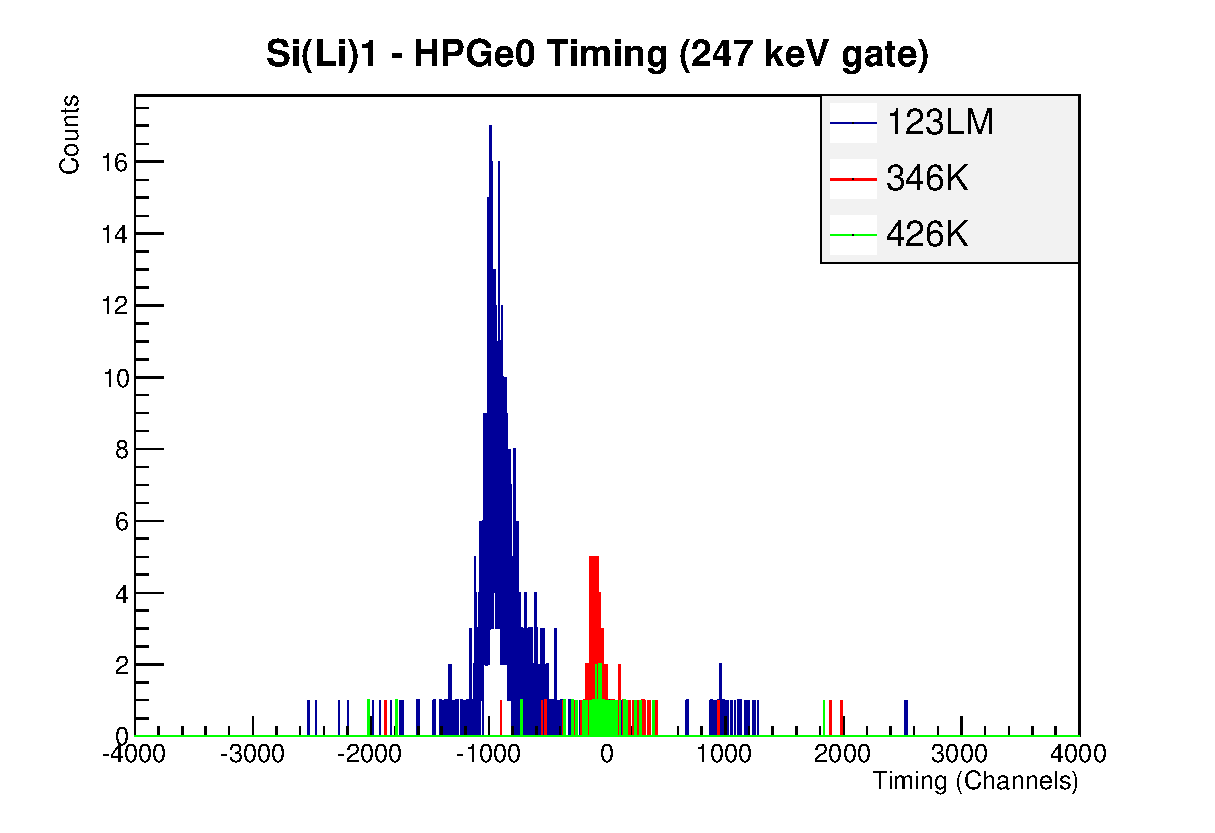
\includegraphics[scale=0.7]{Analysis_Figs/TimingvEnergy.eps}
    \caption[Timing example for the GEORGINA setup]{A plot of the energy-gated timing for a HPGe-Si(Li) detector pairing. The HPGe detector was gated at 247.9 keV, one of the ground state band transitions in the $^{145}$Gd nucleus. The conversion electrons for other transitions in the ground state band were gated on in the Si(Li) detector. Plotted here are the time differences between the two detectors when both peaks were seen in the respective detectors. The 123LM peak was used instead of the K peak due to the high threshold of this detector. As can be seen, the timing has an energy dependence. This dependence is most prominent at lower energies.}
    \label{fig:timing_georgina}
\end{figure}

In the Clovershare data, the timing was done within the electronics, leading to an clean structure, seen in Figure \ref{fig:timing_clover}. Although the same code structure was used for the timing, the gates were all the same within the Clovershare data. The main gate used was $\pm0.3$ and the background ranged from 0.3 to 0.9, using the same scaling as seen in Figure \ref{fig:timing_clover}.

\begin{figure}
    \centering
    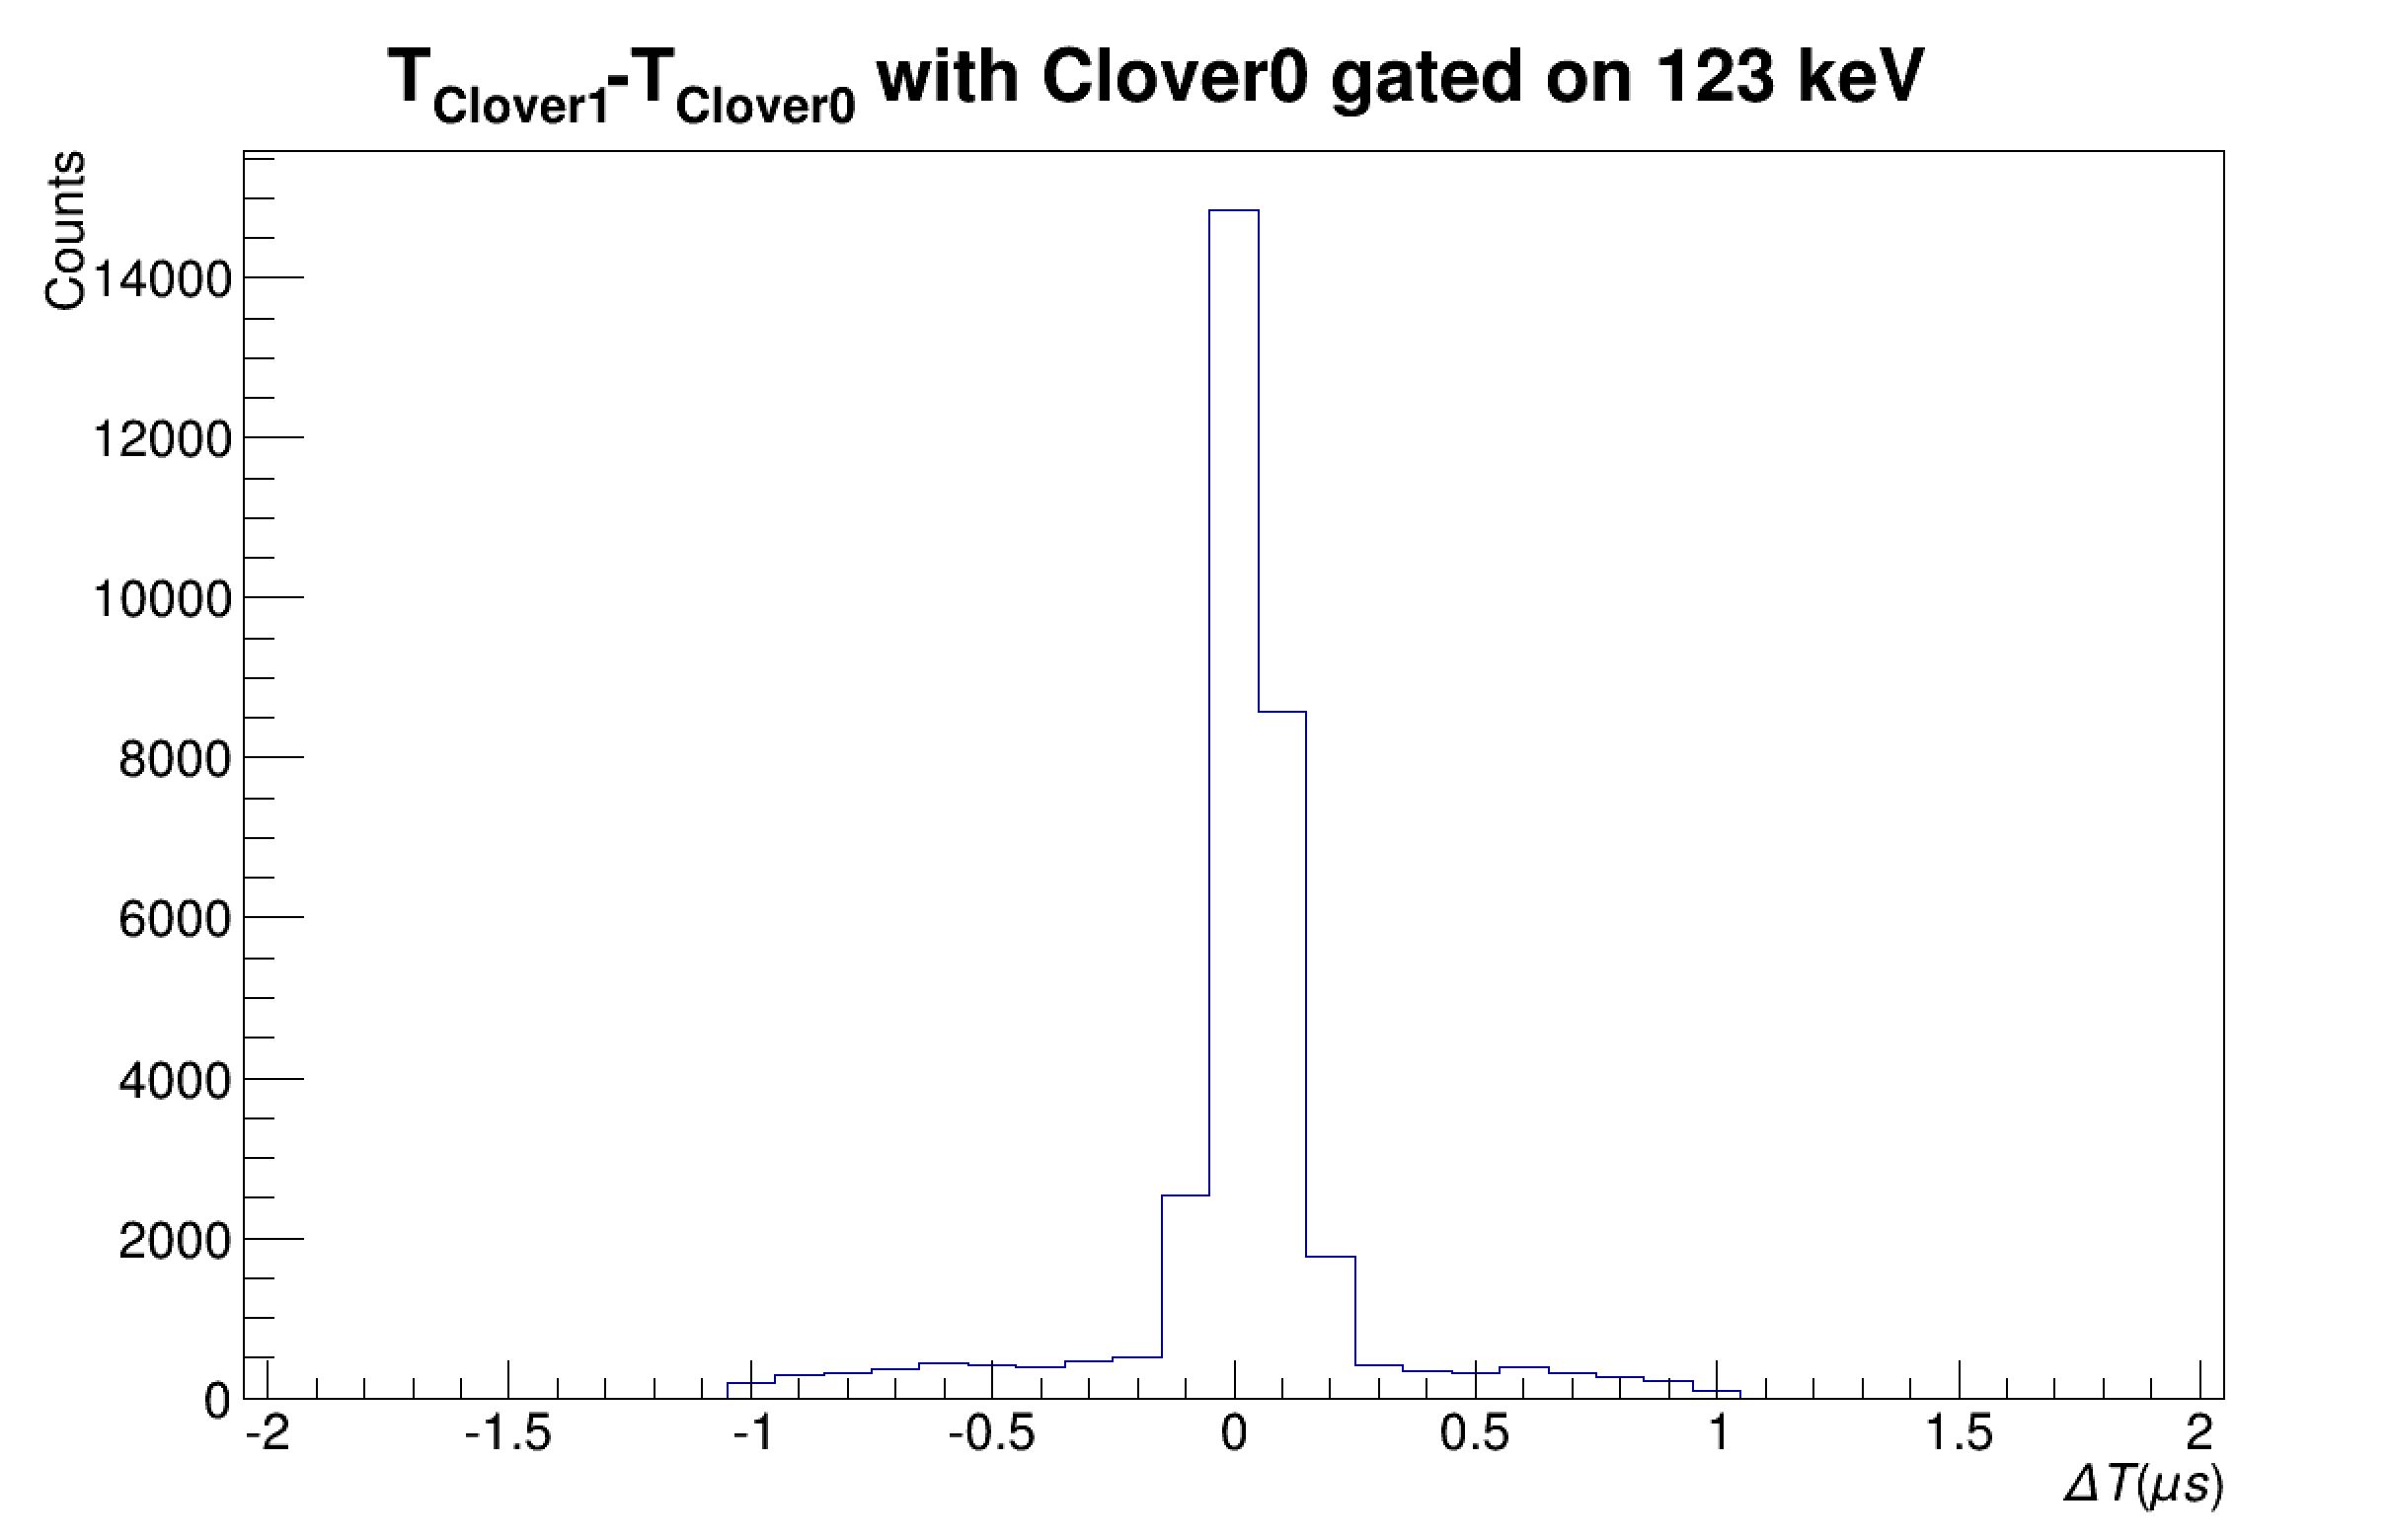
\includegraphics[scale=0.3]{Analysis_Figs/timing_clover.png}
    \caption{Timing between two of the Clovershare detectors, with one detector gated on 123 keV, the lowest transition in the ground state band of $^{154}$Gd. In this data, the gates all looked similarly symmetric, and the timing gates did not need to be varied as they had for the GEORGINA set up.}
    \label{fig:timing_clover}
\end{figure}

Background was taken into account via the energy and timing background gates. The energy background ($E_b$) gate would be subtracted off the main energy gate ($E$). These two energy gates were repeated with the main timing($t$), and background timing($t_b$). The resulting $E-E_b$ spectra, one on the main timing gate, and one on the background timing gate, were then also subtracted as $t-t_b$ to remove any random coincidence from the timing gate.

\section{Systematic Effects}

Several systematic effects had to be taken into account at various stages of analysis. Each will be discussed in further detail in this section. At the calibration stage, there are two major corrections in the Clovershare data. The first, as discussed in section \ref{sec:clover_cal}, is due to the integral non-linearities of the electronics. Second, the instability of the Clovershare detectors required a run-by-run calibration correction. 

In the analysis stage, corrections on extracted values needed to be done based on the angular correlations due to the detectors being at different angles relative to each other. If the angle between the two HPGe detectors were the same as the angle between the HPGe detector and Si(Li) detector(s), this correction would divide out and be unneeded.

\subsection{Electronics-based Integral Non-Linearities}
\label{sec:non-linearity}

There are two kinds of non-linearities from electronics: integral and differential \citep{knoll00:rad_det_meas}. These two non-linearities are interrelated. Integral linearity is most easily seen in the energy calibration. Differential non-linearity can be seen by looking at the count rate with respect to channel number. Generally, the non-linearity can be expressed in calibration by a higher order correction to an otherwise linear calibration. In the GEORGINA detectors, this was the case. In the Clovershare detectors, this was not the case. 

The Pixie-16 MCA used in the Clovershare experiments has non-linearity specifications for 12-bit and 14-bit modes, but not 16-bit, according to the XIA datasheet \citep{xia:_pixie}. These are listed in terms of the difference of the least significant bit (LSB). In an ideal ADC, this number is 0, meaning the difference between two adjacent channels is exactly one LSB. A larger number means the gap is that much greater than one, and a negative number is that much less. When such non-linearities exist, a best case scenario is for the difference to be constant, leading to the polynomial correction. In the case of the Clovershare experiments, the LSB difference between channels does not appear to be constant.

Plotting the residuals of the calibration after doing a linear fit shows what appears to be a sawtooth pattern to the energy points, as seen in Figure \ref{fig:Clover_ene_res}. To fit this sawtooth pattern, it was assumed that the upward slope of the various sections was the same, and the sections were connected via the error function and complimentary error function, to allow for smoothing of the discontinuity. This results in the function
\begin{equation}
    \begin{aligned}
    	E_{res}= m*x+b_1*Erfc\left(\frac{x-f_1}{c}\right)+b_2*Erf\left(\frac{x-f_1}{c}\right)*\\Erfc\left(\frac{x-f_2}{c}\right)+b_3*Erfc\left(\frac{x-f_2}{c}\right)
    \end{aligned}
\end{equation}
where $m$ is the slope, $b_i$ are the various intercepts to shift the correction, $f_i$ is the location of the shift, and $c$ is the curvature of the error function.

\subsection{Run-based Calibration Corrections}

Run-by-run corrections are usually needed when there is drift or instability in the electronics or pre-amplifier. In the Si(Li) and GEORGINA detectors, there was no noticeable drift. The Clovershare data does appear to need a correction for the HPGe detectors. The best way to track these instabilities was to look at known lines in each run, and plot the residuals after calibration, compared to the known value. This can be seen in Figure \ref{fig:clover_run}.  Several well defined peaks were taken in run to define a linear correction for each run. These linear corrections were done on top of the original energy calibration and correction.

\begin{figure}
    \centering
    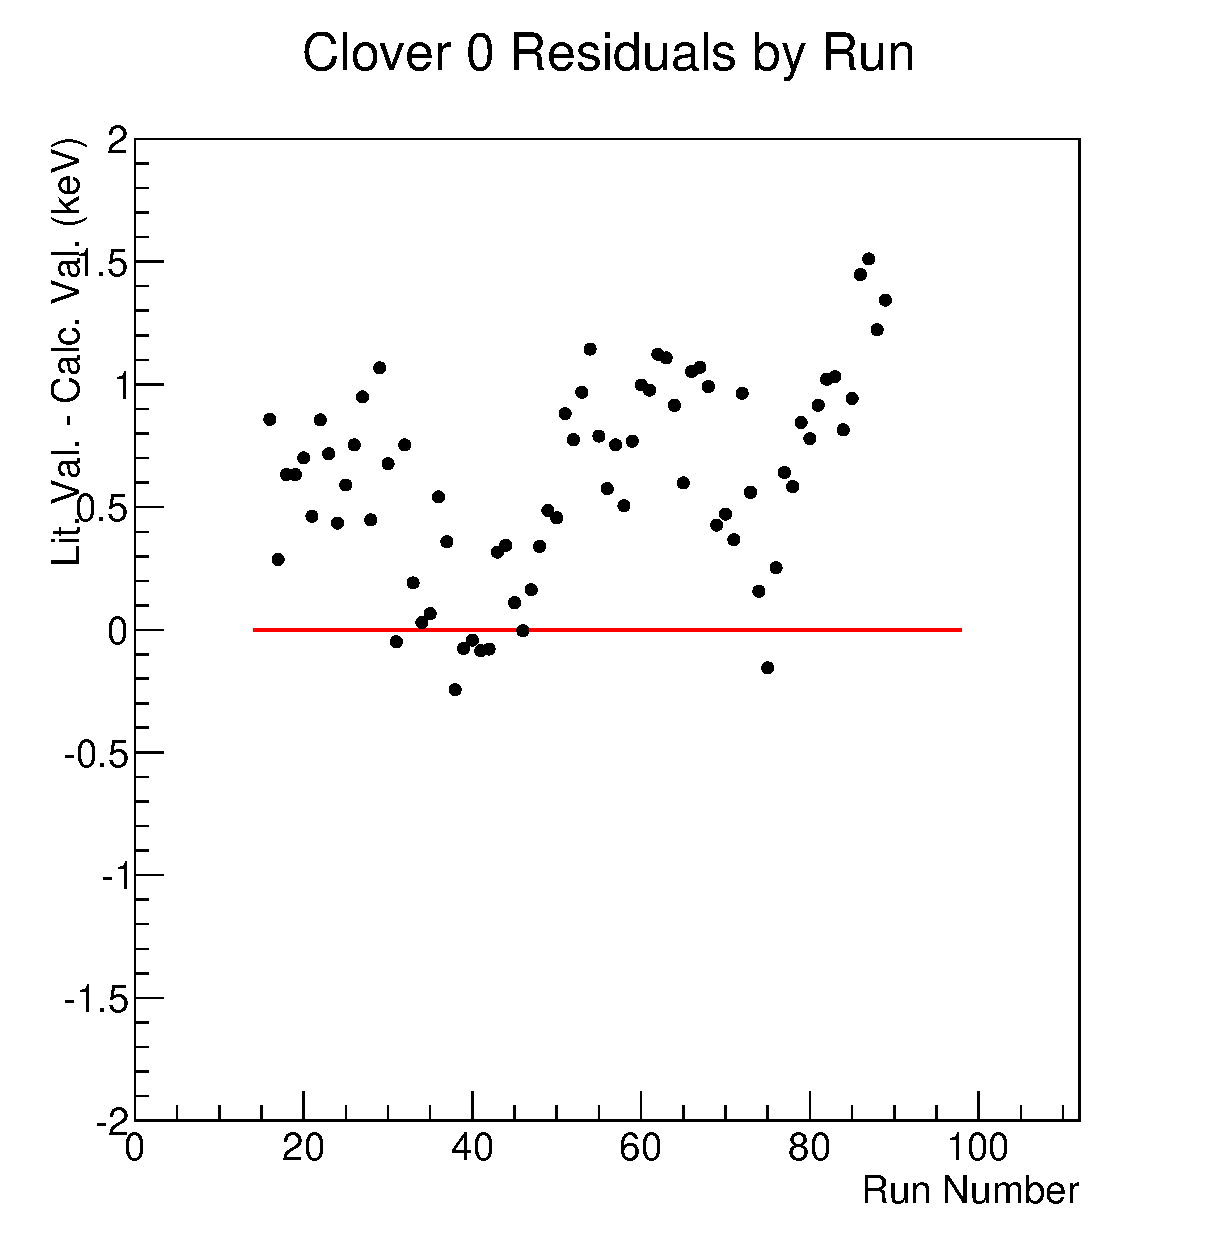
\includegraphics[scale=0.6]{Analysis_Figs/residual_by_run.eps}
    \caption[Example of calibration drift by run.]{The difference between the literature value and the calibrated value (before run-by-run correction) of the naturally occurring $^{40}$K background peak at 1460 keV, plotted by run for one leaf of one HPGe detector. The red line shows $\Delta E=0$.}
    \label{fig:clover_run}
\end{figure}

The peaks used for the run-by-run correction were a combination of the ground-state band peaks in the isotope of interest at low energies, and background gammas at higher energies, such as 1460 keV from $^{40}$K and 1764 keV from $^{214}$Bi. These are naturally occurring from the concrete walls of the NSL.

\subsection{Angular Distributions and Angular Correlations}
\label{sec:angular}

Angular correlations are a well studied phenomenon that arises when trying to look at two types of radiation in coincidence. A thorough exploration of different radiation pairings is explored in \citep{biedenharn53:_theory_angular_corr}. For this work, the pairings of interest are $\gamma-\gamma$ and $\gamma-e$. Triple correlations were also explored, as there were several cases where the intermediate transition was not seen. 

Because the detectors are at different angles with respect to each other, when computing conversion coefficients, or subtracting off conversion electrons from the ground state band within the spectra, a correlation must be made based on these relative angles. Table \ref{tab:rel_angle_g} lists these angles from the ICEBall-Georgina setup, with respect to Detector 1. 

These angles can be calculated using
\begin{equation}
    \theta ' = cos^{-1}(\frac{sin\theta_1 cos\phi_1 sin\theta_2 cos\phi_2 +cos\theta_1 cos\phi_1 cos\theta_2 cos\phi_2 + sin\phi_1 sin\phi_2}{\sqrt{2}})
    \label{eq:rel_angle}
\end{equation}
with the previous definitions given for the angles in Tables \ref{tab:ICE_Det_Loc} and \ref{tab:GEORGE_Det_Loc}.

\begin{table}[]
    \centering
    \caption{Relative Angles of Detectors}
    \begin{tabular}{c|c} \toprule
         Detector & $\theta '$  \\
         \hline 
         HPGe 2 & 180 \\
         SiLi 1 & 90\\
         SiLi 2 & 90\\
         SiLi 3 & 122.5\\
         SiLi 4 & 110.7\\
         SiLi 5 & 69.3 \\
         SiLi 6 & 57.3 \\ \bottomrule
    \end{tabular}
    \footnotesize
    \item Relative angles of the detectors with respect to HPGe 1 in the ICEBall-GEORGINA set up. The angles were calculated using Tables \ref{tab:ICE_Det_Loc} and \ref{tab:GEORGE_Det_Loc} and equation \ref{eq:rel_angle}. All angles are in degrees.
    \label{tab:rel_angle_g}
\end{table}

Angular correlation functions for $\gamma-\gamma$ are usually written as a series of Legendre polynomials, multiplied by a correlation coefficient $A_\nu$, or
\begin{equation}
    w(\beta) = \sum_\nu A_\nu P_\nu(cos\beta)
    \label{eq:ge_corr}
\end{equation}
In the case of $\gamma-e$ correlations, the equation becomes 
\begin{equation}
    \begin{split}
        w_m(\beta) = \sum_\nu b_\nu(LLm) A_\nu P_\nu(cos\beta), \\
        w_e(\beta) = \sum_\nu b_\nu(L+1,L+1,e) A_\nu P_\nu(cos\beta)
        \label{eq:e_corr}
    \end{split}
\end{equation}
depending on if the radiation is electric or magnetic in nature. The $b_\nu$ values are based off the same matrix elements used to calculate theoretical conversion coefficients, and are well understood\citep{rose51:_internal_conversion, rose52:_internal_conversion}.

Both of these cases assume pure multipole transitions. In the case of mixed transitions, the correlation function becomes
\begin{equation}
    W = w_I + \delta^2 w_{II} + 2\delta w_{III}
    \label{eq:mixed_corr}
\end{equation}
where $w_I$ and $w_{II}$ are the pure multipole correlation functions, and $w_{III}$ is a correlation mixing the two multipoles. The variable $\delta$ is known as the mixing ratio. 

These correlations can be further extrapolated to look at cases not just of direct correlations, but of indirect correlations, such as three $\gamma$-rays in cascade. If the middle radiation is not observed, the first and third radiations still have a determinable correlation. This is derived for pure multipoles by \citep{biedenharn53:_theory_angular_corr} and for mixed transitions by \citep{rose53:_angular_corr_supp,osborn53:_angular_corr_3}.

For the experiments in this text, the ratios of these angular correlations at the detectors respective angles is needed to adjust for angular effects. Thus, the ratio becomes a factor, $C_{\angle}$, the ratio of the Si(Li) detector angle to the HPGe detector angle with respect to the detector gated on. The conversion coefficient is divided by this factor for correction.

In the singles, a similar value, based on the angular distribution instead of the angular correlation, must be used for correction. Correlations rise out of the angular distribution caused by the multipolarity of different types of radiation, so the angular distribution can also factor into the singles data, with the beam direction acting as the origin angle, making $C_{\angle}$, the ratio of the Si(Li) detector angle to the HPGe detector angle with respect to the beam axis.

The correction must further be adjusted by the solid angle the detector subtends. Only the azimuthal angle of the detector changes the distribution, so integration over slices of the detector with respect to angle can give a weighted average, i.e.
\begin{equation}
    \overline{W}=\frac{1}{\pi r^2}\int^{tan^{-1}(r/d)}_{-tan^{-1}(r/d)}W(\eta+\omega)\left[2\sqrt{r^2-\left(d\times tan(\omega)\right)^2}\right]\frac{d\delta\omega}{cos^2(\omega)}
\end{equation}
where $W(\theta)$ is the angular distribution function, $\eta$ is the azimuthal angle center of the detector, $d$ is the distance of the detector from the target, and $r$ is the radius of the detector, in the same units as $d$. For the Si(Li) detectors, these distances were taken as the maximal coverage of the mini-orange filters, and the distance between the target and the center of the blocker.  Compared to treating the detectors as points, the effects were small, but the solid angle values were used in the singles.

\section{Upper Limits}
\label{sec:upper_limit}

In $^{156}$Gd, there were several possible transitions of interest at energies less than 250 keV. In that energy range, the ground-state band transitions cover much of the spectrum. Some transitions could be removed through the use of gating on gamma-rays of parallel transitions, but not all the transitions could be removed. This was due, in part, to the gate transitions being in sequence with some of the ground-state band. 

To get an upper limit for the transitions of interest, the ground state band transitions that were in sequence with the gate transition were subtracted off of the conversion electron spectrum through the following method. An example of this subtraction can be seen in Figure \ref{fig:subtraction}. The skewed gaussian fitting function described earlier was given parameters derived from the data and subtracted from the conversion electron spectrum.

\begin{figure}
    \centering
    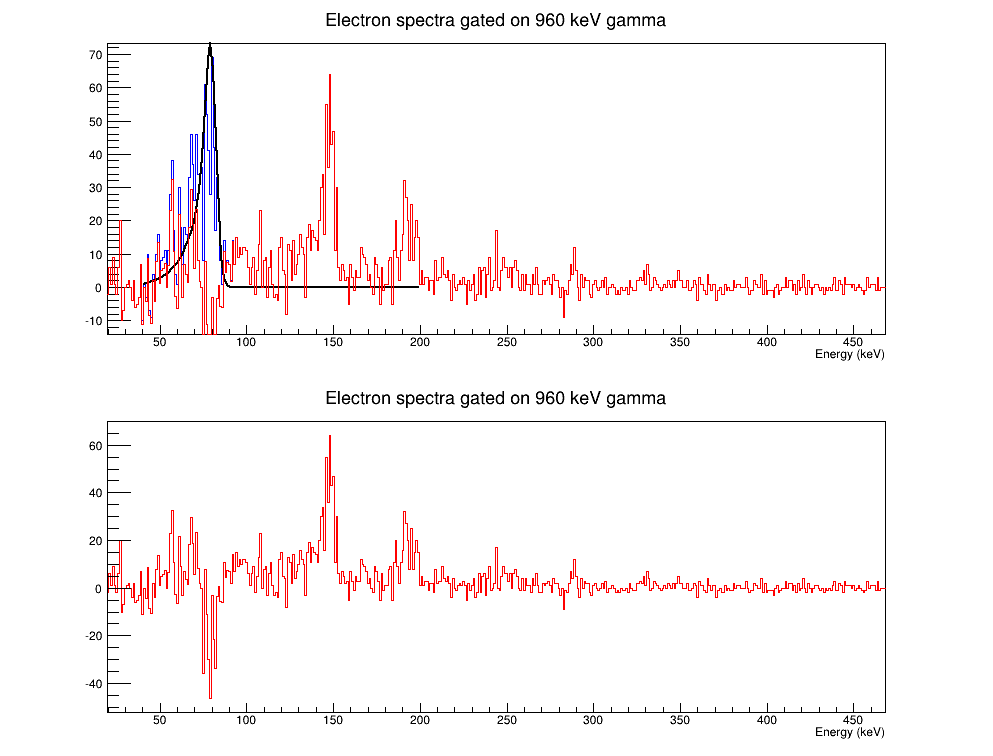
\includegraphics[scale=0.4]{Analysis_Figs/Subtraction_SiLiAll_960.png}
    \caption{An example of the subtraction used to removed the ground state band peaks from spectra. To subtract the conversion electron peak off, the area of the corresponding gamma peak was taken from the same gate. Using the conversion coefficient and the efficiencies of both detectors, the area of the peak could be calculated. From there, this value, along with fixed $R$, $\beta$, $\sigma$, and centroid were used to subtract the peak off. The black line is the function used for subtraction. The blue line is the original spectrum, and the red liine is after subtraction. This code can be found in Appendix \ref{chap:macros}.}
    \label{fig:subtraction}
\end{figure}

The area of the skewed gaussian is obtained by getting the area of the gamma peak, and adjusting by several factors: efficiencies ($\epsilon$), conversion coefficient ($\alpha$, as derived from theory), and correlation coefficients ($W$). This gives the following:
\begin{equation}
    A_{ce} = A_{\gamma}\times\frac{\epsilon_{ce}}{\epsilon_{\gamma}}\times\alpha\times\frac{W_{ce}}{W_{\gamma}}.
    \label{eq:subt_area_skew}
\end{equation}
The height of the skewed gaussian can be derived in terms of the area, $R$, $\sigma$ and $\beta$ to be
\begin{equation}
    H = A\frac{100}{2*e^{-\frac{\sigma^2}{2\beta^2}}R\sigma-\sqrt{2\pi}(R-100)\sigma};
    \label{eq:subt_height_skew}
\end{equation}
These three variables are all unique to the detector, and come directly from fitting the calibration data, as previously discussed. From there, the parameters can be fed into the equation, along with the centroid of the peak, and subtracted directly off the spectrum. Any remaining counts are counted by taking sections on either side of the area of interest and using a global linear fit for the background, as seen in Figure \ref{fig:piecewise}. This linear fit is subtracted off bin-by-bin in the region of interest. The remaining area is then taken as an upper limit on the transition of interest.

\begin{figure}
    \centering
    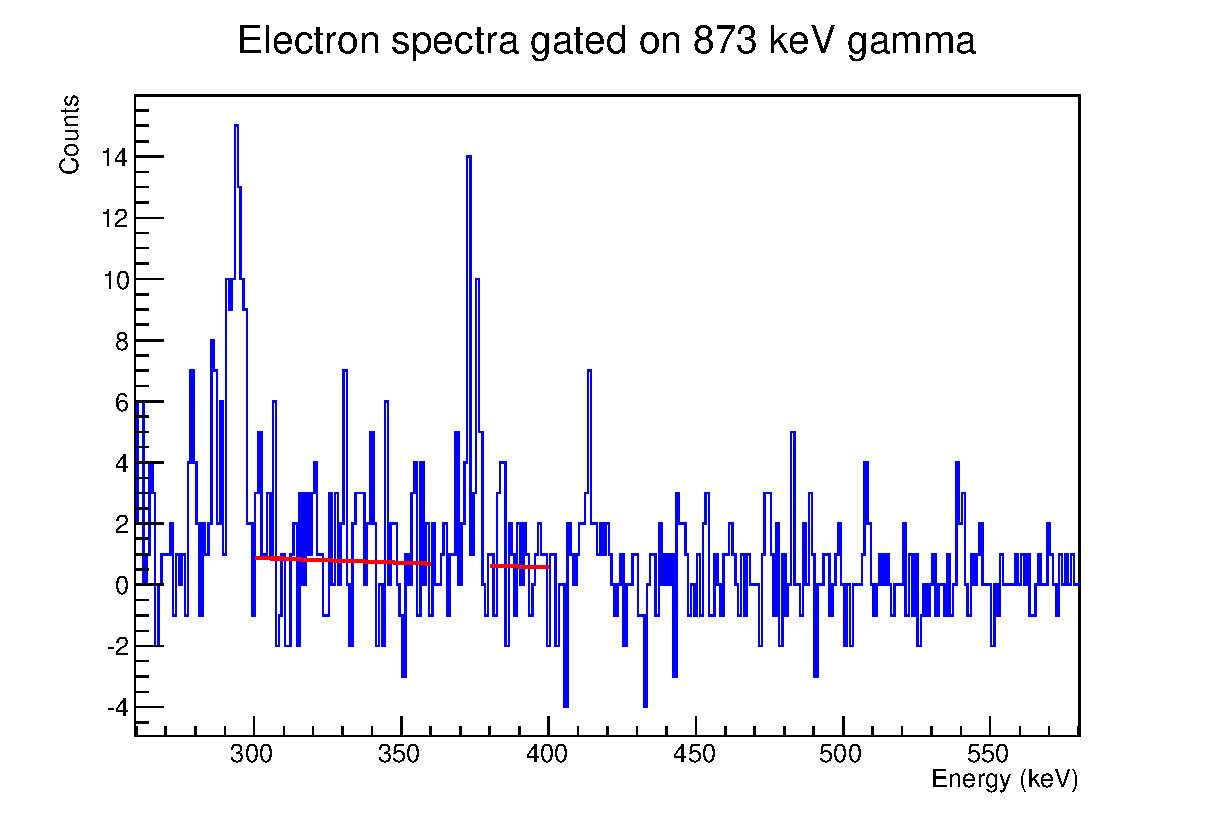
\includegraphics[scale=0.6]{Analysis_Figs/Piecewise_example.eps}
    \caption{An example of the global background fit used for peaks that could not be fit using the skewed gaussian function. The areas on either side of the peak are selected by the user. Once the background fit is done, the central area between the two sections is treated as the peak and the background is subtracted off to give a peak area. The red line shows the fit for the background area, and the two sections used for the background fit. See \ref{chap:macros} for the global-fit function used.}
    \label{fig:piecewise}
\end{figure}

\section{Error Analysis}

When areas of peaks were found, the error is found with the fit. In the cases of the peaks that needed to be fit by estimating the background and subtracting it off, the error of the area is assumed to be the square root of the counts in the peak added in quadrature with the error in the background.

These areas are propagated through calculations via the equation
\begin{equation}
    \sigma_{f}^2=\sum_{i}\left(\sigma_{x_i}\frac{\delta f}{\delta_{x_i}}\right)^2
\end{equation}
where $f$ is a function of all $x_i$ in the sum \citep{bevington03:_error}. If the function is related to all variables via some form of a polynomial, i.e. $(x_i)^a$ where $a$ is a constant, then it can be rewritten as
\begin{equation}
    \sigma_{f}^2=f*\sum_{i}\left(\frac{\sigma_{x_i}}{a*x_i}\right)^2
\end{equation}
Errors on the areas of both gamma-rays and electrons were propagated through the data. The error on the efficiency was estimated by shifting the efficiency value $\pm0.5\sigma$ and calculating upper and lower limit functions for the efficiency. 

In the final results, the uncertainties were kept separate into statistical and systematic effects. Statistical effects are caused by the areas of the peaks. Systematic effects are from the uncertainty in the efficiency of both the HPGe and Si(Li) detectors, as well as an uncertainty in the angular correlations, based on the solid angle covered by the detectors.